\documentclass[11pt,a4paper]{article}

\usepackage[margin=2.5cm]{geometry}
\usepackage{amsmath,amssymb}
\usepackage{graphicx}
\usepackage{listings}
\usepackage{xcolor}
\usepackage{fontspec}
\setmonofont{JetBrains Mono}[Scale=0.9]
\usepackage{tikz}
\usetikzlibrary{arrows.meta,decorations.markings}
\usepackage[skip=6pt plus 2pt]{parskip}
\usepackage[hidelinks]{hyperref}

\definecolor{codebg}{HTML}{F6F8FA}
\definecolor{codeframe}{HTML}{D0D7DE}
\definecolor{codekw}{HTML}{CF222E}
\definecolor{codestr}{HTML}{0A3069}
\definecolor{codecom}{HTML}{6E7781}
\definecolor{codenum}{HTML}{8C959F}
\definecolor{codefn}{HTML}{8250DF}
\lstset{
  language=Python,
  basicstyle=\ttfamily\fontsize{6.5}{7.5}\selectfont,
  backgroundcolor=\color{codebg},
  keywordstyle=\color{codekw}\bfseries,
  stringstyle=\color{codestr},
  commentstyle=\color{codecom}\itshape,
  numbers=left,
  numberstyle=\tiny\color{codenum},
  breaklines=true,
  frame=single,
  rulecolor=\color{codeframe},
  showstringspaces=false,
  columns=fullflexible,
  keepspaces=true,
  morekeywords={self},
  emph={True,False,None},
  emphstyle=\color{codefn},
}

\title{JPEG Compression of a 24\,bpp Image}
\author{Sahithyan K. \\ 230557T}
\date{\today}

\begin{document}
\maketitle

\section{Introduction}

JPEG is a lossy compression method for continuous-tone still images such as photographs. This report describes how the baseline JPEG encoder compresses a 24\,bpp image, with a worked example and a Python implementation.

\subsection{Terms}

\begin{itemize}
\item bpp\\
  Bits per pixel. A 24\,bpp image stores 3 channels (red, green, blue) of 8 bits each per pixel.
\item Lossless compression\\
  The decoder recovers the original data exactly.
\item Lossy compression\\
  The decoder recovers an approximation of the original. Information the viewer is unlikely to notice is discarded to reduce size.
\item Compression ratio\\
  Original size divided by compressed size.
\item PSNR\\
  Peak signal-to-noise ratio. A measure, in decibels (dB), of how close a decoded image is to the original. Higher means closer. See Section~\ref{sec:psnr}.
\item JPEG\\
  Joint Photographic Experts Group. The name refers to the committee and to the standard it wrote, published as ITU-T T.81 \cite{t81}.
\item Baseline JPEG\\
  The standard's basic mode, where the image is encoded in a single pass with Huffman coding and 8 bits per channel. The standard also defines progressive, hierarchical and lossless modes. This report covers only baseline.
\item JFIF\\
  JPEG File Interchange Format \cite{jfif}. A minimal file format that wraps JPEG data.
\item DCT\\
  Discrete cosine transform. A transform from pixel values to spatial frequency coefficients \cite{ahmed1974}.
\item Huffman coding\\
  A variable-length code that gives shorter bit strings to more frequent symbols \cite{huffman1952}.
\end{itemize}

\subsection{History}

\begin{itemize}
\item 1952\\
  Huffman publishes his minimum-redundancy code \cite{huffman1952}.
\item 1974\\
  Ahmed, Natarajan and Rao introduce the DCT \cite{ahmed1974}.
\item 1986\\
  ISO and CCITT (now ITU-T) form the Joint Photographic Experts Group to define a standard for still image compression \cite{wallace1992}.
\item 1992\\
  The standard is published as ITU-T T.81 \cite{t81}. ISO adopts it as ISO/IEC 10918-1 in 1994.
\item 1992\\
  Eric Hamilton of C-Cube Microsystems publishes JFIF 1.02 \cite{jfif}.
\end{itemize}

The T.81 standard specifies how image data is compressed. It does not fix the color space, the pixel aspect ratio or the file layout. JFIF fills this gap by requiring YCbCr for color images and defining a header with the pixel density. Files with the \texttt{.jpg} or \texttt{.jpeg} extension are normally JFIF files.

\subsection{Alternatives to JFIF}

JFIF is not the only way to store JPEG data. The alternatives wrap the same compressed data with different metadata.
\begin{itemize}
\item Exif\\
  Exchangeable image file format \cite{exif}. Used by digital cameras and phones. Stores camera settings, timestamps and GPS location. Most photos from cameras are Exif files, not JFIF files.
\item SPIFF\\
  Still Picture Interchange File Format, defined in ITU-T T.84 \cite{t84}. Intended to replace JFIF, with support for more color spaces and bit depths. Rarely used.
\end{itemize}
The compressed image data is the same in all 3 formats. Most software reads JFIF and Exif files alike.

\subsection{Motivation}

A $1920\times1080$ image at 24\,bpp takes $1920\times1080\times3=6{,}220{,}800$ bytes, about 5.9\,MiB, when stored raw. JPEG commonly reaches compression ratios of 10:1 or more with little visible loss \cite{wallace1992}.

\pagebreak

\section{Processing Steps}\label{sec:steps}

The baseline JPEG encoder \cite{wallace1992} compresses a 24\,bpp image (3 channels of 8 bits per pixel) in 7 steps, shown in Figure~\ref{fig:pipeline}. Only chroma subsampling and quantization discard information by design.

\begin{figure}[h]
\centering
\begin{tabular}{c}
RGB image $\rightarrow$ color conversion $\rightarrow$ chroma subsampling
$\rightarrow$ 8$\times$8 blocks + DCT \\
$\rightarrow$ quantization $\rightarrow$ zigzag, RLE, Huffman coding $\rightarrow$ \texttt{.jpg}
\end{tabular}
\caption{Baseline JPEG encoder.}
\label{fig:pipeline}
\end{figure}

\subsection{Color Space Conversion}

YCbCr separates luma (brightness) from chroma (color). Human vision resolves brightness detail better than color detail, so the 2 can be compressed differently. R, G and B each mix both, so they cannot. JFIF \cite{jfif} defines the conversion:
\begin{align*}
Y   &= 0.299\,R + 0.587\,G + 0.114\,B \\
C_b &= 128 - 0.168736\,R - 0.331264\,G + 0.5\,B \\
C_r &= 128 + 0.5\,R - 0.418688\,G - 0.081312\,B
\end{align*}
Here:
\begin{itemize}
\item $R, G, B$: 8-bit red, green and blue values
\item $Y$: luma
\item $C_b$: blue-difference chroma
\item $C_r$: red-difference chroma
\end{itemize}

\subsection{Chroma Subsampling}

Chroma subsampling stores $C_b$ and $C_r$ with fewer samples than $Y$. Human vision is less sensitive to color detail than to brightness detail, so the loss is rarely visible \cite{gonzalez}. $Y$ is never subsampled.

Every pixel always keeps its own $Y$ sample. The schemes differ only in how many $C_b$ and $C_r$ samples are kept. The name $J{:}a{:}b$ describes a block 4 pixels wide and 2 pixels tall.
\begin{itemize}
\item $J$: pixels per row, always 4
\item $a$: chroma samples in the first row
\item $b$: new chroma samples in the second row
\end{itemize}
A value of $b=0$ does not mean the second row has no color. The second row reuses the chroma samples of the first row.

Common schemes:
\begin{itemize}
\item 4:4:4\\
  $a=4$, $b=4$. Each of the 8 pixels has its own chroma sample. No subsampling.
\item 4:2:2\\
  $a=2$, $b=2$. Each chroma sample covers 2 pixels side by side. Each row has 2 samples, giving 4 in total.
\item 4:2:0\\
  $a=2$, $b=0$. Each chroma sample covers a $2\times2$ group of pixels. The 2 samples in the first row serve both rows, giving 2 in total. JPEG encoders use this by default.
\end{itemize}
Samples needed for the $4\times2$ block, counting $Y$, $C_b$ and $C_r$:
\begin{center}
\begin{tabular}{lcccc}
Scheme & $Y$ & $C_b$ & $C_r$ & Total \\
\hline
4:4:4 & 8 & 8 & 8 & 24 \\
4:2:2 & 8 & 4 & 4 & 16 \\
4:2:0 & 8 & 2 & 2 & 12 \\
\end{tabular}
\end{center}
4:2:0 needs half the samples of 4:4:4.

Figure~\ref{fig:subsampling} shows where the samples sit in each scheme.

\newcommand{\pixgrid}[2]{%
  \draw[gray] (#1,0) grid (#1+4,2);
  \foreach \x in {0,...,3} \foreach \y in {0,1} \fill (#1+\x+0.5,\y+0.5) circle (0.07);
  \node at (#1+2,-0.5) {#2};}
\begin{figure}[h]
\centering
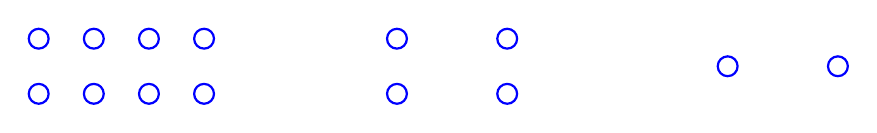
\begin{tikzpicture}[scale=0.7]
\pixgrid{0}{4:4:4}
\foreach \x in {0,...,3} \foreach \y in {0,1}
  \draw[blue,thick] (\x+0.5,\y+0.5) circle (0.18);
\pixgrid{6}{4:2:2}
\foreach \x in {1,3} \foreach \y in {0,1}
  \draw[blue,thick] (6+\x,\y+0.5) circle (0.18);
\pixgrid{12}{4:2:0}
\foreach \x in {1,3}
  \draw[blue,thick] (12+\x,1) circle (0.18);
\end{tikzpicture}
\caption{Sample positions in a $4\times2$ pixel block. Black dots are $Y$ samples. Blue circles are shared $C_b$ and $C_r$ samples.}
\label{fig:subsampling}
\end{figure}

A $16\times16$ region reduces from $3\times256=768$ samples to $256+64+64=384$ in the same way. The data halves before any other compression step.

Example with 4:2:0, using a $4\times4$ region of $C_b$ values. The region has 4 groups of $2\times2$ pixels.

\[
\begin{bmatrix}
100&102&110&112\\
 98&104&108&114\\
 90& 92&120&118\\
 94& 96&122&124
\end{bmatrix}
\]

Averages:
\begin{itemize}
\item Top-left group\\
  $(100+102+98+104)/4=101$
\item Top-right group\\
  $(110+112+108+114)/4=111$
\item Bottom-left group\\
  $(90+92+94+96)/4=93$
\item Bottom-right group\\
  $(120+118+122+124)/4=121$
\end{itemize}
Each group is replaced by its average, so 16 values become 4.
\[
\begin{bmatrix}
100&102&110&112\\
 98&104&108&114\\
 90& 92&120&118\\
 94& 96&122&124
\end{bmatrix}
\longrightarrow
\begin{bmatrix}
101&111\\
 93&121
\end{bmatrix}
\]
The decoder restores the original size by copying each value into its $2\times2$ group.
\[
\begin{bmatrix}
101&101&111&111\\
101&101&111&111\\
 93& 93&121&121\\
 93& 93&121&121
\end{bmatrix}
\]
The error (original minus restored) is:
\[
\begin{bmatrix}
-1& 1&-1& 1\\
-3& 3&-3& 3\\
-3&-1&-1&-3\\
 1& 3& 1& 3
\end{bmatrix}
\]

The largest error is 3 on a scale of 255, which is not visible to the human eye. The original values cannot be recovered.

The same happens to $C_r$. For these $4\times4$ pixels, the 48 samples ($Y$, $C_b$, $C_r$ at 16 each) reduce to $16+4+4=24$.

\subsection{Block Splitting and Level Shift}

Each channel is split into $8\times8$ blocks. Edges are padded by repeating the last row or column when a dimension is not a multiple of 8. Each sample then has 128 subtracted, which moves the range to $[-128, 127]$ and centers it on 0. The result is called a \textbf{level-shifted sample}:
\[
f(x,y)=p(x,y)-2^{P-1}
\]
where $p(x,y)$ is the pixel value and $P$ is the bit depth ($P=8$ here). The decoder adds 128 back at the end.

Every later step runs on each block independently. Heavy compression therefore leaves visible block edges, called blocking artifacts.

\subsection{Discrete Cosine Transform}

The 2D discrete cosine transform (DCT) \cite{ahmed1974} rewrites an $8\times8$ block as a weighted sum of 64 fixed cosine patterns of increasing spatial frequency.

\[
F(u,v)=\tfrac14\,C(u)C(v)\sum_{x=0}^{7}\sum_{y=0}^{7}
f(x,y)\cos\frac{(2x+1)u\pi}{16}\cos\frac{(2y+1)v\pi}{16}
\]
Here:
\begin{itemize}
\item $f(x,y)$: level-shifted sample at row $x$, column $y$
\item $F(u,v)$: coefficient for the pattern of vertical frequency $u$ and horizontal frequency $v$
\item $C(0)=1/\sqrt2$
\item $C(k)=1$ for $k>0$
\end{itemize}

The coefficient $F(0,0)$ is the \textbf{DC coefficient}. It is proportional to the block average. The other 63 coefficients are \textbf{AC coefficients}. The level shift is applied to zero-center the data. This transformation reduces the block average and the DC coefficient. AC coefficients are unchanged. 

The DCT is invertible, apart from rounding error.

In natural images, neighboring pixels usually have similar values. A block therefore varies slowly. It is described mostly by smooth, low-frequency patterns. Most of its information ends up in a few coefficients near $F(0,0)$. The 64 coefficients form an $8\times8$ array, indexed by $u$ (row) and $v$ (column). These low-frequency coefficients sit at the top-left of that array. The coefficients toward the bottom-right represent fast, fine detail. They are usually close to 0.

\begin{figure}[h]
\centering
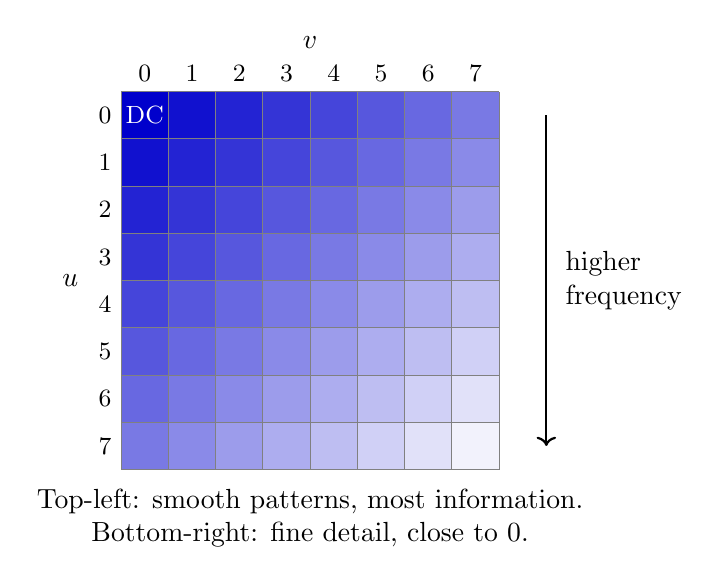
\begin{tikzpicture}[scale=0.6]
\foreach \u in {0,...,7} \foreach \v in {0,...,7}
  \fill[blue!80!black, opacity={1-(\u+\v)/14*0.95}] (\v,-\u-1) rectangle (\v+1,-\u);
\draw[gray] (0,-8) grid (8,0);
\node[white] at (0.5,-0.5) {\small DC};
\foreach \k in {0,...,7} {
  \node[above] at (\k+0.5,0) {\small \k};
  \node[left] at (0,-\k-0.5) {\small \k};}
\node[above] at (4,0.7) {$v$};
\node[left] at (-0.7,-4) {$u$};
\draw[->,thick] (9,-0.5) -- (9,-7.5);
\node[right,align=left] at (9.2,-4) {higher\\frequency};
\node[below,align=center] at (4,-8.2) {Top-left: smooth patterns, most information.\\Bottom-right: fine detail, close to 0.};
\end{tikzpicture}
\caption{The $8\times8$ array of DCT coefficients $F(u,v)$. Darker cells hold larger coefficients in a typical block.}
\label{fig:dct-array}
\end{figure}

\subsection{Quantization}

Quantization divides each coefficient by the matching entry of a table $Q$ and rounds to an integer.
\[
F_q(u,v)=\operatorname{round}\!\left(\frac{F(u,v)}{Q(u,v)}\right)
\]
Low frequencies get small divisors. High frequencies get large ones. Most high-frequency coefficients therefore round to 0. This rounding is the main irreversible loss in JPEG. The quality setting scales $Q$. A larger $Q$ gives a smaller file and more visible damage.

The $Y$ channel uses one table. The $C_b$ and $C_r$ channels use a second table with larger divisors. The eye is less sensitive to fine color detail than to fine brightness detail, so chroma can be rounded harder. The standard luminance table from Annex K of ITU-T T.81 \cite{t81} is:
\[
Q=\begin{bmatrix}
16&11&10&16& 24& 40& 51& 61\\
12&12&14&19& 26& 58& 60& 55\\
14&13&16&24& 40& 57& 69& 56\\
14&17&22&29& 51& 87& 80& 62\\
18&22&37&56& 68&109&103& 77\\
24&35&55&64& 81&104&113& 92\\
49&64&78&87&103&121&120&101\\
72&92&95&98&112&100&103& 99
\end{bmatrix}
\]

\subsection{Zigzag Scan and Run-Length Coding}

The \textbf{zigzag scan} reads a quantized block diagonally from $(0,0)$ to $(7,7)$. Coefficients come out ordered from low to high frequency, which groups the zeros at the end. A single end-of-block (EOB) symbol replaces the trailing zeros.

\begin{figure}[h]
\centering
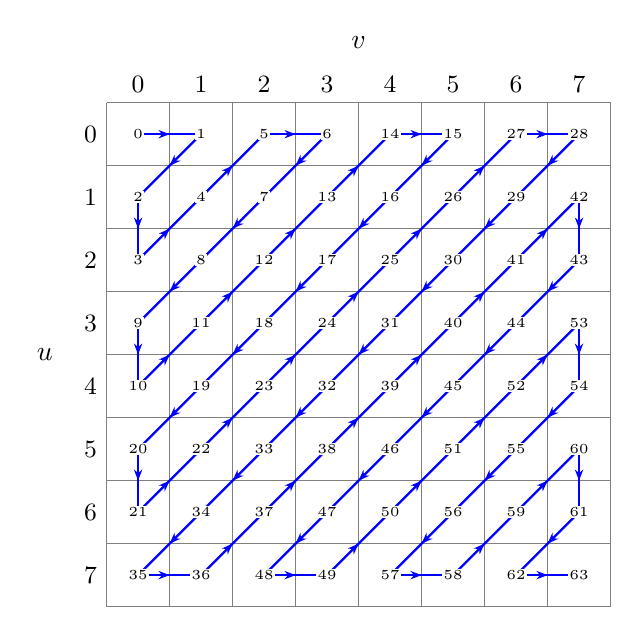
\begin{tikzpicture}[scale=0.8]
\draw[gray] (0,-8) grid (8,0);
\tikzset{seg/.style={blue,thick,postaction={decorate},decoration={markings,mark=at position 0.5 with {\arrow{Stealth[length=4pt]}}}}}
\draw[seg] (0.5,-0.5) -- (1.5,-0.5);
\draw[seg] (1.5,-0.5) -- (0.5,-1.5);
\draw[seg] (0.5,-1.5) -- (0.5,-2.5);
\draw[seg] (0.5,-2.5) -- (1.5,-1.5);
\draw[seg] (1.5,-1.5) -- (2.5,-0.5);
\draw[seg] (2.5,-0.5) -- (3.5,-0.5);
\draw[seg] (3.5,-0.5) -- (2.5,-1.5);
\draw[seg] (2.5,-1.5) -- (1.5,-2.5);
\draw[seg] (1.5,-2.5) -- (0.5,-3.5);
\draw[seg] (0.5,-3.5) -- (0.5,-4.5);
\draw[seg] (0.5,-4.5) -- (1.5,-3.5);
\draw[seg] (1.5,-3.5) -- (2.5,-2.5);
\draw[seg] (2.5,-2.5) -- (3.5,-1.5);
\draw[seg] (3.5,-1.5) -- (4.5,-0.5);
\draw[seg] (4.5,-0.5) -- (5.5,-0.5);
\draw[seg] (5.5,-0.5) -- (4.5,-1.5);
\draw[seg] (4.5,-1.5) -- (3.5,-2.5);
\draw[seg] (3.5,-2.5) -- (2.5,-3.5);
\draw[seg] (2.5,-3.5) -- (1.5,-4.5);
\draw[seg] (1.5,-4.5) -- (0.5,-5.5);
\draw[seg] (0.5,-5.5) -- (0.5,-6.5);
\draw[seg] (0.5,-6.5) -- (1.5,-5.5);
\draw[seg] (1.5,-5.5) -- (2.5,-4.5);
\draw[seg] (2.5,-4.5) -- (3.5,-3.5);
\draw[seg] (3.5,-3.5) -- (4.5,-2.5);
\draw[seg] (4.5,-2.5) -- (5.5,-1.5);
\draw[seg] (5.5,-1.5) -- (6.5,-0.5);
\draw[seg] (6.5,-0.5) -- (7.5,-0.5);
\draw[seg] (7.5,-0.5) -- (6.5,-1.5);
\draw[seg] (6.5,-1.5) -- (5.5,-2.5);
\draw[seg] (5.5,-2.5) -- (4.5,-3.5);
\draw[seg] (4.5,-3.5) -- (3.5,-4.5);
\draw[seg] (3.5,-4.5) -- (2.5,-5.5);
\draw[seg] (2.5,-5.5) -- (1.5,-6.5);
\draw[seg] (1.5,-6.5) -- (0.5,-7.5);
\draw[seg] (0.5,-7.5) -- (1.5,-7.5);
\draw[seg] (1.5,-7.5) -- (2.5,-6.5);
\draw[seg] (2.5,-6.5) -- (3.5,-5.5);
\draw[seg] (3.5,-5.5) -- (4.5,-4.5);
\draw[seg] (4.5,-4.5) -- (5.5,-3.5);
\draw[seg] (5.5,-3.5) -- (6.5,-2.5);
\draw[seg] (6.5,-2.5) -- (7.5,-1.5);
\draw[seg] (7.5,-1.5) -- (7.5,-2.5);
\draw[seg] (7.5,-2.5) -- (6.5,-3.5);
\draw[seg] (6.5,-3.5) -- (5.5,-4.5);
\draw[seg] (5.5,-4.5) -- (4.5,-5.5);
\draw[seg] (4.5,-5.5) -- (3.5,-6.5);
\draw[seg] (3.5,-6.5) -- (2.5,-7.5);
\draw[seg] (2.5,-7.5) -- (3.5,-7.5);
\draw[seg] (3.5,-7.5) -- (4.5,-6.5);
\draw[seg] (4.5,-6.5) -- (5.5,-5.5);
\draw[seg] (5.5,-5.5) -- (6.5,-4.5);
\draw[seg] (6.5,-4.5) -- (7.5,-3.5);
\draw[seg] (7.5,-3.5) -- (7.5,-4.5);
\draw[seg] (7.5,-4.5) -- (6.5,-5.5);
\draw[seg] (6.5,-5.5) -- (5.5,-6.5);
\draw[seg] (5.5,-6.5) -- (4.5,-7.5);
\draw[seg] (4.5,-7.5) -- (5.5,-7.5);
\draw[seg] (5.5,-7.5) -- (6.5,-6.5);
\draw[seg] (6.5,-6.5) -- (7.5,-5.5);
\draw[seg] (7.5,-5.5) -- (7.5,-6.5);
\draw[seg] (7.5,-6.5) -- (6.5,-7.5);
\draw[seg] (6.5,-7.5) -- (7.5,-7.5);
\node[font=\tiny,fill=white,inner sep=0.5pt] at (0.5,-0.5) {0};
\node[font=\tiny,fill=white,inner sep=0.5pt] at (1.5,-0.5) {1};
\node[font=\tiny,fill=white,inner sep=0.5pt] at (0.5,-1.5) {2};
\node[font=\tiny,fill=white,inner sep=0.5pt] at (0.5,-2.5) {3};
\node[font=\tiny,fill=white,inner sep=0.5pt] at (1.5,-1.5) {4};
\node[font=\tiny,fill=white,inner sep=0.5pt] at (2.5,-0.5) {5};
\node[font=\tiny,fill=white,inner sep=0.5pt] at (3.5,-0.5) {6};
\node[font=\tiny,fill=white,inner sep=0.5pt] at (2.5,-1.5) {7};
\node[font=\tiny,fill=white,inner sep=0.5pt] at (1.5,-2.5) {8};
\node[font=\tiny,fill=white,inner sep=0.5pt] at (0.5,-3.5) {9};
\node[font=\tiny,fill=white,inner sep=0.5pt] at (0.5,-4.5) {10};
\node[font=\tiny,fill=white,inner sep=0.5pt] at (1.5,-3.5) {11};
\node[font=\tiny,fill=white,inner sep=0.5pt] at (2.5,-2.5) {12};
\node[font=\tiny,fill=white,inner sep=0.5pt] at (3.5,-1.5) {13};
\node[font=\tiny,fill=white,inner sep=0.5pt] at (4.5,-0.5) {14};
\node[font=\tiny,fill=white,inner sep=0.5pt] at (5.5,-0.5) {15};
\node[font=\tiny,fill=white,inner sep=0.5pt] at (4.5,-1.5) {16};
\node[font=\tiny,fill=white,inner sep=0.5pt] at (3.5,-2.5) {17};
\node[font=\tiny,fill=white,inner sep=0.5pt] at (2.5,-3.5) {18};
\node[font=\tiny,fill=white,inner sep=0.5pt] at (1.5,-4.5) {19};
\node[font=\tiny,fill=white,inner sep=0.5pt] at (0.5,-5.5) {20};
\node[font=\tiny,fill=white,inner sep=0.5pt] at (0.5,-6.5) {21};
\node[font=\tiny,fill=white,inner sep=0.5pt] at (1.5,-5.5) {22};
\node[font=\tiny,fill=white,inner sep=0.5pt] at (2.5,-4.5) {23};
\node[font=\tiny,fill=white,inner sep=0.5pt] at (3.5,-3.5) {24};
\node[font=\tiny,fill=white,inner sep=0.5pt] at (4.5,-2.5) {25};
\node[font=\tiny,fill=white,inner sep=0.5pt] at (5.5,-1.5) {26};
\node[font=\tiny,fill=white,inner sep=0.5pt] at (6.5,-0.5) {27};
\node[font=\tiny,fill=white,inner sep=0.5pt] at (7.5,-0.5) {28};
\node[font=\tiny,fill=white,inner sep=0.5pt] at (6.5,-1.5) {29};
\node[font=\tiny,fill=white,inner sep=0.5pt] at (5.5,-2.5) {30};
\node[font=\tiny,fill=white,inner sep=0.5pt] at (4.5,-3.5) {31};
\node[font=\tiny,fill=white,inner sep=0.5pt] at (3.5,-4.5) {32};
\node[font=\tiny,fill=white,inner sep=0.5pt] at (2.5,-5.5) {33};
\node[font=\tiny,fill=white,inner sep=0.5pt] at (1.5,-6.5) {34};
\node[font=\tiny,fill=white,inner sep=0.5pt] at (0.5,-7.5) {35};
\node[font=\tiny,fill=white,inner sep=0.5pt] at (1.5,-7.5) {36};
\node[font=\tiny,fill=white,inner sep=0.5pt] at (2.5,-6.5) {37};
\node[font=\tiny,fill=white,inner sep=0.5pt] at (3.5,-5.5) {38};
\node[font=\tiny,fill=white,inner sep=0.5pt] at (4.5,-4.5) {39};
\node[font=\tiny,fill=white,inner sep=0.5pt] at (5.5,-3.5) {40};
\node[font=\tiny,fill=white,inner sep=0.5pt] at (6.5,-2.5) {41};
\node[font=\tiny,fill=white,inner sep=0.5pt] at (7.5,-1.5) {42};
\node[font=\tiny,fill=white,inner sep=0.5pt] at (7.5,-2.5) {43};
\node[font=\tiny,fill=white,inner sep=0.5pt] at (6.5,-3.5) {44};
\node[font=\tiny,fill=white,inner sep=0.5pt] at (5.5,-4.5) {45};
\node[font=\tiny,fill=white,inner sep=0.5pt] at (4.5,-5.5) {46};
\node[font=\tiny,fill=white,inner sep=0.5pt] at (3.5,-6.5) {47};
\node[font=\tiny,fill=white,inner sep=0.5pt] at (2.5,-7.5) {48};
\node[font=\tiny,fill=white,inner sep=0.5pt] at (3.5,-7.5) {49};
\node[font=\tiny,fill=white,inner sep=0.5pt] at (4.5,-6.5) {50};
\node[font=\tiny,fill=white,inner sep=0.5pt] at (5.5,-5.5) {51};
\node[font=\tiny,fill=white,inner sep=0.5pt] at (6.5,-4.5) {52};
\node[font=\tiny,fill=white,inner sep=0.5pt] at (7.5,-3.5) {53};
\node[font=\tiny,fill=white,inner sep=0.5pt] at (7.5,-4.5) {54};
\node[font=\tiny,fill=white,inner sep=0.5pt] at (6.5,-5.5) {55};
\node[font=\tiny,fill=white,inner sep=0.5pt] at (5.5,-6.5) {56};
\node[font=\tiny,fill=white,inner sep=0.5pt] at (4.5,-7.5) {57};
\node[font=\tiny,fill=white,inner sep=0.5pt] at (5.5,-7.5) {58};
\node[font=\tiny,fill=white,inner sep=0.5pt] at (6.5,-6.5) {59};
\node[font=\tiny,fill=white,inner sep=0.5pt] at (7.5,-5.5) {60};
\node[font=\tiny,fill=white,inner sep=0.5pt] at (7.5,-6.5) {61};
\node[font=\tiny,fill=white,inner sep=0.5pt] at (6.5,-7.5) {62};
\node[font=\tiny,fill=white,inner sep=0.5pt] at (7.5,-7.5) {63};
\foreach \k in {0,...,7} {
  \node[above] at (\k+0.5,0) {\small \k};
  \node[left] at (0,-\k-0.5) {\small \k};}
\node[above] at (4,0.7) {$v$};
\node[left] at (-0.7,-4) {$u$};
\end{tikzpicture}
\caption{Zigzag scan order of an $8\times8$ block. The path starts at $(0,0)$ and ends at $(7,7)$.}
\label{fig:zigzag}
\end{figure}

DC and AC coefficients are coded differently.
\begin{itemize}
\item DC\\
  The difference from the previous block's DC is stored. Neighboring blocks have similar averages, so the differences are small.
\item AC\\
  Each non-zero value is stored as a pair $(r,s)$ followed by the value's bits.
\end{itemize}
Here:
\begin{itemize}
\item $r$: number of zeros before the value
\item $s$: number of bits needed for the value's magnitude
\end{itemize}

\subsection{Huffman Coding}

A Huffman code assigns short bit strings to frequent symbols and long ones to rare symbols. It is applied to the DC difference sizes and the $(r,s)$ pairs. The value bits follow each symbol unchanged. A negative value is stored as the bitwise complement of its magnitude, so $3$ is \texttt{11} and $-3$ is \texttt{00}.

Huffman coding is lossless. The tables are either the standard ones in ITU-T T.81 \cite{t81} or are built per image and stored in the file. The bit stream, with headers holding the image size, $Q$ and the Huffman tables, is the \texttt{.jpg} file \cite{pennebaker1992}.

\subsection{Decoding}

The decoder applies the steps in reverse order:
\begin{itemize}
\item Huffman decoding
\item Inverse zigzag
\item Multiplication by $Q$
\item Inverse DCT
\item Adding 128
\item Chroma upsampling
\item YCbCr to RGB conversion
\end{itemize}
The output approximates the original. Subsampling and quantization cannot be inverted.

\subsection{Worked Example}

This example follows the first MCU of the lighthouse image (512$\times$768) at quality 50. The program writes it with \texttt{--trace trace.txt} (\href{https://github.com/sahithyandev/labs/tree/main/s5/image-processing/jpeg-compression/trace.txt}{\texttt{trace.txt}}). Only the first of the six blocks (the top-left $Y$ block) is shown in full.

Color conversion of the pixel $(0,0)$, with $(R,G,B)=(75,93,94)$:
\begin{align*}
Y   &= 22.4 + 54.6 + 10.7 = 87.7 \\
C_b &= 128 - 12.7 - 30.8 + 47.0 = 131.5 \\
C_r &= 128 + 37.5 - 38.9 - 7.6 = 118.9
\end{align*}
$C_b$ and $C_r$ are then averaged over $2\times2$ groups. An MCU covers $16\times16$ pixels and has 4 $Y$ blocks, 1 $C_b$ block and 1 $C_r$ block.

Level-shifted samples of the first $Y$ block, rounded to 1 decimal place:
\[
f-128=\begin{bmatrix}
-40.3&-37.1&-39.1&-36.1&-30.5&-33.2&-33.2&-30.5 \\
-40.3&-39.1&-41.2&-40.1&-37.2&-34.5&-30.5&-33.2 \\
-38.6&-37.3&-40.1&-40.1&-37.2&-34.5&-30.5&-30.5 \\
-30.6&-37.3&-41.4&-40.1&-37.2&-36.1&-31.5&-31.5 \\
-29.3&-36.3&-40.1&-39.1&-39.1&-41.2&-35.5&-33.1 \\
-27.9&-34.7&-39.1&-43.1&-40.4&-38.7&-35.8&-34.7 \\
-31.9&-30.7&-38.5&-36.1&-40.1&-39.1&-36.1&-33.4 \\
-29.1&-31.9&-34.7&-33.5&-34.5&-39.1&-40.1&-39.1
\end{bmatrix}
\]
DCT:
\[
F=\begin{bmatrix}
-288.1&-4.1&15.1&4.4&3.7&-0.6&-3.9&0.5 \\
-0.3&-18.1&-4.3&0.8&-2.8&-1.5&-0.7&1.2 \\
2.9&1.2&-10.0&-2.5&-0.8&-3.2&-0.8&-1.6 \\
-1.1&1.2&2.7&0.1&1.3&-1.0&0.6&0.5 \\
3.0&3.5&-3.4&0.7&4.8&-0.2&0.3&1.2 \\
3.4&-2.3&0.8&-0.6&-0.0&-1.5&-0.7&-1.8 \\
1.0&0.8&-0.8&1.0&-0.2&-1.5&1.9&1.8 \\
0.5&-0.5&-1.3&-3.7&0.7&-0.8&-1.4&-1.4
\end{bmatrix}
\]
Quantization with the luminance $Q$ above:
\[
F_q=\begin{bmatrix}
-18&0&2&0&0&0&0&0 \\
0&-2&0&0&0&0&0&0 \\
0&0&-1&0&0&0&0&0 \\
0&0&0&0&0&0&0&0 \\
0&0&0&0&0&0&0&0 \\
0&0&0&0&0&0&0&0 \\
0&0&0&0&0&0&0&0 \\
0&0&0&0&0&0&0&0
\end{bmatrix}
\]
Only 4 of the 64 values are non-zero. Zigzag scan:
\[
-18,\,0,\,0,\,0,\,-2,\,2,\,\underbrace{0,\dots,0}_{6},\,-1,\,\underbrace{0,\dots,0}_{51}
\]
Symbols, taking the previous DC as 0:
\begin{itemize}
\item DC\\
  Difference $-18$, size 5.
\item AC\\
  $(3,2){:}-2$, $(0,2){:}2$, $(6,1){:}-1$.
\item End\\
  EOB.
\end{itemize}
The 64 values reduce to 1 DC difference, 3 $(r,s)$ pairs and 1 EOB. With the Huffman codes built for this image, the block becomes (code, then value bits):
\begin{center}
\texttt{11110|01101\ \ 11110101|01\ \ 011|10\ \ 111010|0\ \ 010}
\end{center}
which is 35 bits instead of $64\times8=512$ bits for the original samples.

\subsection{PSNR}\label{sec:psnr}

PSNR measures the loss of a lossy codec with a single number. It compares each value of the original image with the same value of the decoded image. The mean squared error (MSE) is
\[
\mathrm{MSE}=\frac{1}{3WH}\sum_{c=1}^{3}\sum_{x=1}^{H}\sum_{y=1}^{W}\bigl(p(x,y,c)-\hat p(x,y,c)\bigr)^2
\]
and the PSNR is
\[
\mathrm{PSNR}=10\log_{10}\frac{255^2}{\mathrm{MSE}}\ \text{dB}
\]
Here:
\begin{itemize}
\item $W, H$: image width and height in pixels
\item $p, \hat p$: original and decoded value of channel $c$ (R, G or B) at the pixel
\item $255$: the largest value of an 8-bit sample, the peak
\end{itemize}
The logarithm turns the error into a scale where each 10\,dB is a tenfold change in MSE. For example, an MSE of 1 gives $10\log_{10}255^2\approx48.1$\,dB, and an MSE of 100 gives 28.1\,dB. Identical images have an MSE of 0 and an infinite PSNR. For 8-bit photos, values above about 40\,dB are hard to tell from the original, and values from 30 to 40\,dB are usually good. PSNR counts every error equally, so it does not match human perception exactly.

\section{Python Implementation}

The encoder and decoder use only the Python standard library, except that Pillow loads the input image. The code follows the steps in Section~\ref{sec:steps}. Three classes hold the code: \texttt{Color} (RGB and YCbCr conversion), \texttt{Matrix} (transpose and matrix product, used by the DCT) and \texttt{Jpeg}. In \texttt{Jpeg}, \texttt{encode} and \texttt{decode} run the steps one after the other and each step is a method. The methods both directions need (DCT, quantization, zigzag, symbols, Huffman codes) are shared.

All files of this assignment (code, tests, test image, trace and this report) are in the \href{https://github.com/sahithyandev/labs/tree/main/s5/image-processing/jpeg-compression}{GitHub repository}, including \href{https://github.com/sahithyandev/labs/tree/main/s5/image-processing/jpeg-compression/JR_230557T.py}{\texttt{JR\_230557T.py}}.

The input is a BMP or PNG file, loaded with Pillow as 24\,bpp RGB (a BMP stores 24\,bpp pixels directly). The encoder writes a real baseline JPEG file: JFIF header, quantization tables, Huffman tables and the scan data, with 4:2:0 subsampling. Any JPEG viewer can open it. The decoder reads such a file back to measure the loss. Run it with:

\texttt{python3 JR\_230557T.py image.bmp [quality]} to compress into \texttt{name-quality.jpg}. It prints the file size, the compression ratio and the PSNR of the decoded result. Adding \texttt{--trace trace.txt} also writes the steps and the data of the first MCU to that file, as a worked example.

\lstinputlisting{JR_230557T.py}

\subsection{Results}

The test image is a 512$\times$768 photo of a lighthouse, which is 9\,437\,184 bits at 24\,bpp. The BMP file is 1\,179\,702 bytes. Figure~\ref{fig:images} shows the original and two compressed versions. Table~\ref{tab:results} shows the size of the JPEG file and the quality of the decoded image at ten quality settings.

A lower quality gives a larger divisor table, so the file shrinks and the PSNR falls. The ratio is the size of the pixel data divided by the size of the JPEG file. Quality 50 already gives a ratio of about 29, and quality 90 a ratio of about 10. Quality 100 gives the largest file and a ratio of only 3.8, because the divisors are all 1 and only rounding loss remains. Decoding the files with the image tools of the operating system gives the same PSNR, which confirms that they are valid JPEG files.

\begin{figure}[h]
\centering
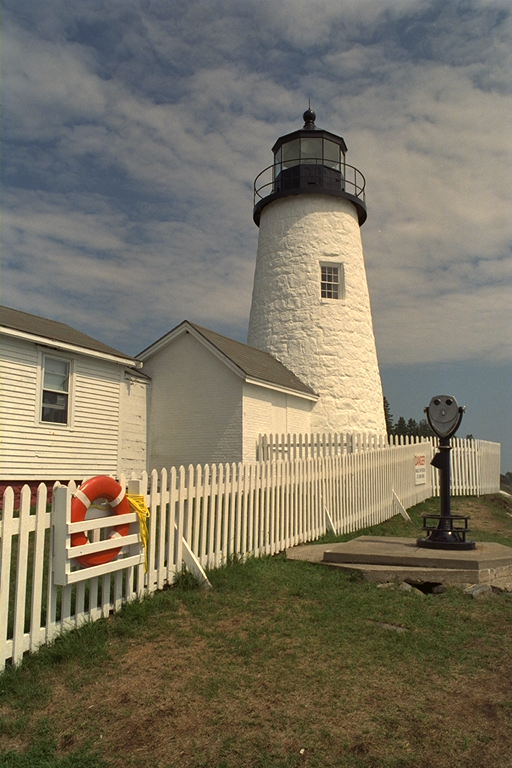
\includegraphics[width=0.32\textwidth]{lighthouse.png}\hfill
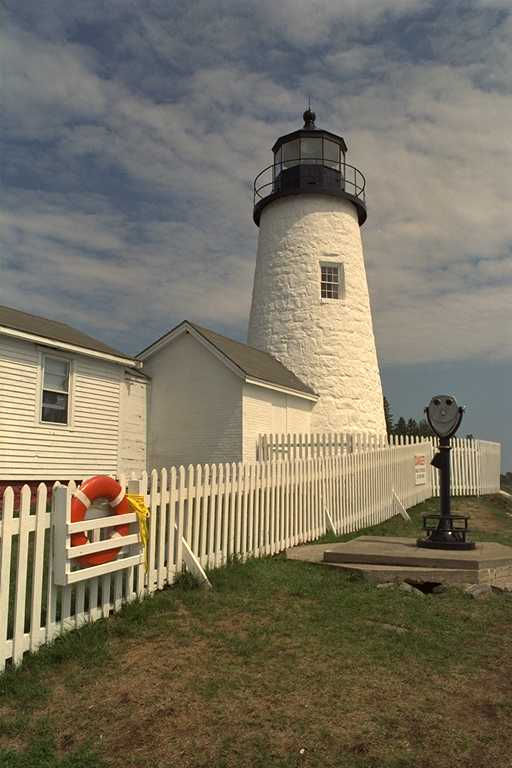
\includegraphics[width=0.32\textwidth]{lighthouse-50.jpg}\hfill
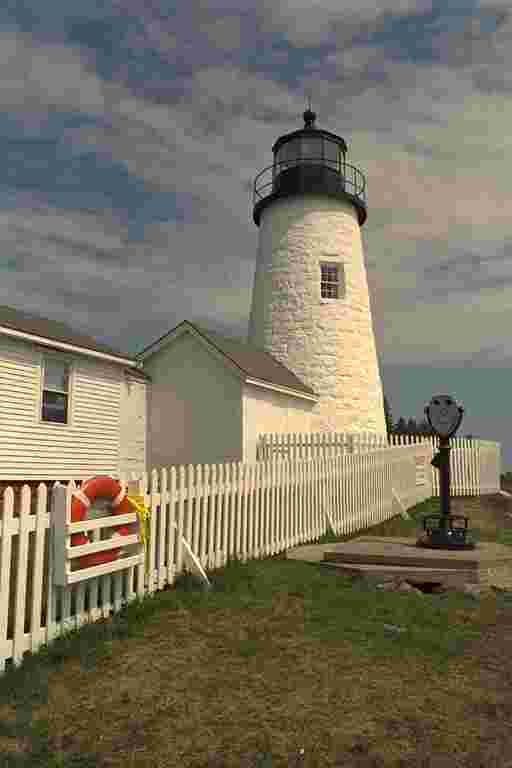
\includegraphics[width=0.32\textwidth]{lighthouse-10.jpg}
\caption{The test image: original (left), quality 50 (middle, 28.6:1) and quality 10 (right, 100.1:1).}
\label{fig:images}
\end{figure}

\begin{table}[h]
\centering
\begin{tabular}{rrrr}
Quality & File size (bytes) & Compression ratio & PSNR (dB) \\
\hline
10 & 11\,788 & 100.1 & 26.8 \\
20 & 20\,997 & 56.2 & 29.3 \\
30 & 28\,814 & 40.9 & 30.6 \\
40 & 35\,261 & 33.5 & 31.6 \\
50 & 41\,297 & 28.6 & 32.3 \\
60 & 47\,826 & 24.7 & 33.0 \\
70 & 57\,674 & 20.4 & 34.0 \\
80 & 74\,276 & 15.9 & 35.4 \\
90 & 112\,754 & 10.5 & 38.1 \\
100 & 312\,866 & 3.8 & 46.1
\end{tabular}
\caption{Compression of the lighthouse image.}
\label{tab:results}
\end{table}

\subsection{Tests}

The tests are in \href{https://github.com/sahithyandev/labs/tree/main/s5/image-processing/jpeg-compression/test_JR_230557T.py}{\texttt{test\_JR\_230557T.py}}. The file contents are not included in this report to keep this short. The tests check for color conversion, the DCT, the quantization, the zigzag order and the run-length symbols, plane operations, the bit coding, the Huffman code and its 16-bit limit, the byte stuffing, the image loader, the PSNR, JPEG file's markers and the stored tables. Encode--decode round trips run on the lighthouse photo and on a small crop of it whose size is not a multiple of 16. Run them with \texttt{python3 -m unittest}. The real-image tests need \texttt{lighthouse.bmp} in the same folder.

{\small
\begin{thebibliography}{9}
\bibitem{wallace1992} G.~K. Wallace, ``The JPEG still picture compression
  standard,'' \emph{IEEE Trans.\ Consumer Electronics}, vol.~38, no.~1,
  pp.~xviii--xxxiv, Feb.\ 1992. \url{https://doi.org/10.1109/30.125072}
\bibitem{t81} ITU-T Recommendation T.81 | ISO/IEC 10918-1, \emph{Digital
  compression and coding of continuous-tone still images: Requirements and
  guidelines}, 1992. \url{https://www.w3.org/Graphics/JPEG/itu-t81.pdf}
\bibitem{jfif} E.~Hamilton, ``JPEG File Interchange Format, Version 1.02,''
  C-Cube Microsystems, Sept.\ 1992. \url{https://www.w3.org/Graphics/JPEG/jfif3.pdf}
\bibitem{ahmed1974} N.~Ahmed, T.~Natarajan and K.~R. Rao, ``Discrete cosine
  transform,'' \emph{IEEE Trans.\ Computers}, vol.~C-23, no.~1, pp.~90--93,
  Jan.\ 1974. \url{https://doi.org/10.1109/T-C.1974.223784}
\bibitem{exif} CIPA, \emph{Exchangeable image file format for digital still
  cameras: Exif Version 2.32}, CIPA DC-008, 2019. \url{https://www.cipa.jp/std/documents/e/DC-X008-Translation-2019-E.pdf}
\bibitem{t84} ITU-T Recommendation T.84 | ISO/IEC 10918-3, \emph{Digital
  compression and coding of continuous-tone still images: Extensions}, 1996. \url{https://www.itu.int/rec/T-REC-T.84}
\bibitem{huffman1952} D.~A. Huffman, ``A method for the construction of
  minimum-redundancy codes,'' \emph{Proc.\ IRE}, vol.~40, no.~9,
  pp.~1098--1101, Sept.\ 1952. \url{https://doi.org/10.1109/JRPROC.1952.273898}
\bibitem{pennebaker1992} W.~B. Pennebaker and J.~L. Mitchell, \emph{JPEG:
  Still Image Data Compression Standard}. New York: Van Nostrand Reinhold,
  1992. \url{https://openlibrary.org/isbn/0442012721}
\bibitem{gonzalez} R.~C. Gonzalez and R.~E. Woods, \emph{Digital Image
  Processing}, 4th ed. Pearson, 2018. \url{https://openlibrary.org/isbn/9780133356724}
\end{thebibliography}
}

\end{document}
